\clearpage
\chapter{Introduction}
In this document, we descripted a full installation of follow components: Firewall, DNS, SSH, Email and Web. As well, we show you all possibilities you can take within the provided script. We let you understand that the components are hardened and give you some thoughts about the future. Everything start with the walkthrough chapter, a complete walkthrough through the scripts explained based on the output. You can quickly and clearly follow up what is happening where and how. There is an overview code directory tree, which indicates all the scripts which are made. After it starts with all the components, which will be installed.
\begin{itemize} 
	\item \textbf{Overview}: This Section is about the main script, which bundles all components. The user also has the possibility to create his individual setup and if necessary to perform uninstallation and modifications on a second run.
	\item \textbf{Firewall}:The firewall can be extended with additional rules with the help of a configuration file. The file can be found in the ``files'' directory under the name ``fw.conf''.
	\item \textbf{DNS}: In the DNS part, two DNS servers will be installed. Both are from nlnetlabs: unbound and NSD. Unbound is used as resolver, to handle all requests from this server and NSD is used as authoritative name server. Such a separation increases security.
	\item \textbf{User management}: Since some services also require Unix users, scripts have been written to make it easier to create and assign users to services. Both the mail part and the SSH part need such users.
	\item \textbf{SSH}: The SSH part is not only about making the server more secure by forbidding the root user to log in, but also about equipping new or existing users with right and ssh keys so that a login is still possible via specific users.
	\item \textbf{Email}: A secure mail server with postfix is set up in the email part. Unix users are also required here.
	\item \textbf{Web}: In the web part nginx and apache are used. The nginx is used as reverse proxy and the apache as frontend webserver.
\end{itemize}

Results are important, so the hardening Tests section is about giving you a feeling about what one can expect from a successful complete run of the script. Based on common hardening pages and tools, tests were made to show how secure the server is, before the script and after a complete run of the scripts. 
\begin{itemize} 
	\item \textbf{Firewall}: The firewall tests were performed with nmap. The results of the firewall test can seem a bit irritating at first: more ports are open than before. However, this makes sense, because certain ports are needed by the services. What is open or closed before also depends on the host of the server.
	\item \textbf{DNS}: It was important not only to make a DNS secure, but also to make it  independent. With the own resolver this was very successful and so the user of the scripts has a DNS detached from big companies like Google or Cloudflare.
	\item \textbf{SSH}: Apart from forbidding the root user from logging in, we also made sure that after the SSH configuration only algorithms are used that are currently considered as secure.
	\item \textbf{Mail}: With secure protocols and antispam measures, the mail server was configured so that it received very good marks during the tests. We tested it with https://emailsecuritygrader.com and https://www.hardenize.com.
	\item \textbf{Web}: Also the web part could be tested via https://www.hardenize.com .  There we also achieved very good values.
\end{itemize}
In addition, you will find a small step-by-step guide (currently only macOS guide) to set up the email client to work with your server. Moreover, in the conclusion we discuss about extended functionalities like multiple domains / e-mail addresses, more hardening possibilities, containerization and code migration. At the very end, you find all configured config files of each component.


\section{Prerequisits}
In order to start a complete run of the scripts, it is worth making some things ready in advance so that the run can go clean and fast.

\subsection{Ubuntu 18.04 Server}
You need your own Ubuntu Server (Version 18.04), which is an accessible from the internet. You need root access.

\subsection{Domain}
You need your own domain. A free test domain can easily be found with a small search in any web search engine. 

\subsection{Minimal Linux knowledge}
The script is in command line only, so you need some minimal Linux knowledge. You should know how to navigate and execute a command inside the terminal.

\newpage
\section{Architecture overview}
Here you see a simple architecture overview, how your server will look like, if you install all the components.

\begin{figure}[H]
	\centering
	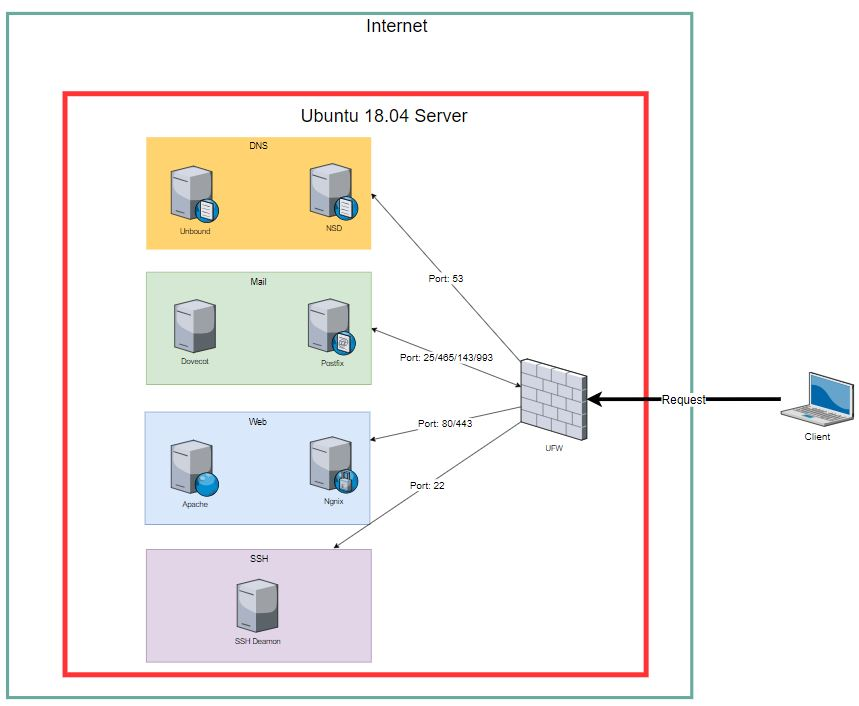
\includegraphics[width=0.9\linewidth]{diagram/overview_diagramm.JPG}
	\caption{Architecture overview}
	\label{fig:beforeWeb}
\end{figure}
